\documentclass[twoside, 11pt]{article}
\usepackage{aaai24}
\usepackage{amsmath}
\usepackage{amssymb}
\usepackage{enumitem}
\usepackage{graphicx}
\usepackage{listings}
\usepackage{xcolor}
\usepackage{diagbox}
\usepackage{array}
\setcounter{MaxMatrixCols}{20}
\setlength{\arraycolsep}{5pt}
% \renewcommand{\arraystretch}{1.5}
% The file aaai24.sty is the official AAAI 2024 style file
% You can find it on the AAAI 2024 website or in the template provided


\sloppy\begin{document}

\title{CIFAR-10 Image Classification using ResNet Architecture}
\author{Sudharshan Ramesh, sr7431 || 
Mohammed Hamid, mh7483\\
\texttt{Github: https://github.com/exploring-curiosity/DeepLearning-CIFAR-10}}
\maketitle

\begin{abstract}

    The project was done as part of Deep Learning Course in NYU, for using ResNet architecture to classify CIFAR-10 images. The CIFAR-10 dataset consists of 60,000 32x32 color images in 10 classes, with 6,000 images per class (50,000 train and 10,000 test images). We implemented a ResNet model to classify these images and achieved an accuracy of 92.48\% on the test set. The project involved data preprocessing, model implementation, training, hyper-parameter tuning, fine tuning and evaluation.
\end{abstract}

\section{Overview}
\label{sec:intro}
In this project, we aim to develop an image classification model for the CIFAR-10 dataset using the ResNet architecture, while ensuring the model remains efficient with fewer than 5 million parameters. The CIFAR-10 dataset consists of 60,000 32x32 color images across 10 distinct classes, making it a popular benchmark for evaluating classification models in computer vision.

The ResNet architecture, known for its use of residual connections, enables the training of deep networks by mitigating the vanishing gradient problem. In this project, we adapt the ResNet model for CIFAR-10 classification and focus on optimizing the neural network’s structure to meet the constraint of 5 million parameters. This involves adjusting the depth and width of the network, as well as experimenting with variations in the residual block designs to maintain model performance while ensuring computational efficiency.

\section{Methodology}
\label{sec:method}
We aimed to design an efficient ResNet architecture for CIFAR-10 image classification while ensuring the total number of parameters remained under 5 million. The process was iterative, beginning with the standard ResNet-18 architecture, which initially contains around 11 million parameters, and subsequently refining it to achieve a compact yet high-performing model.
\subsection{Architecture Design}
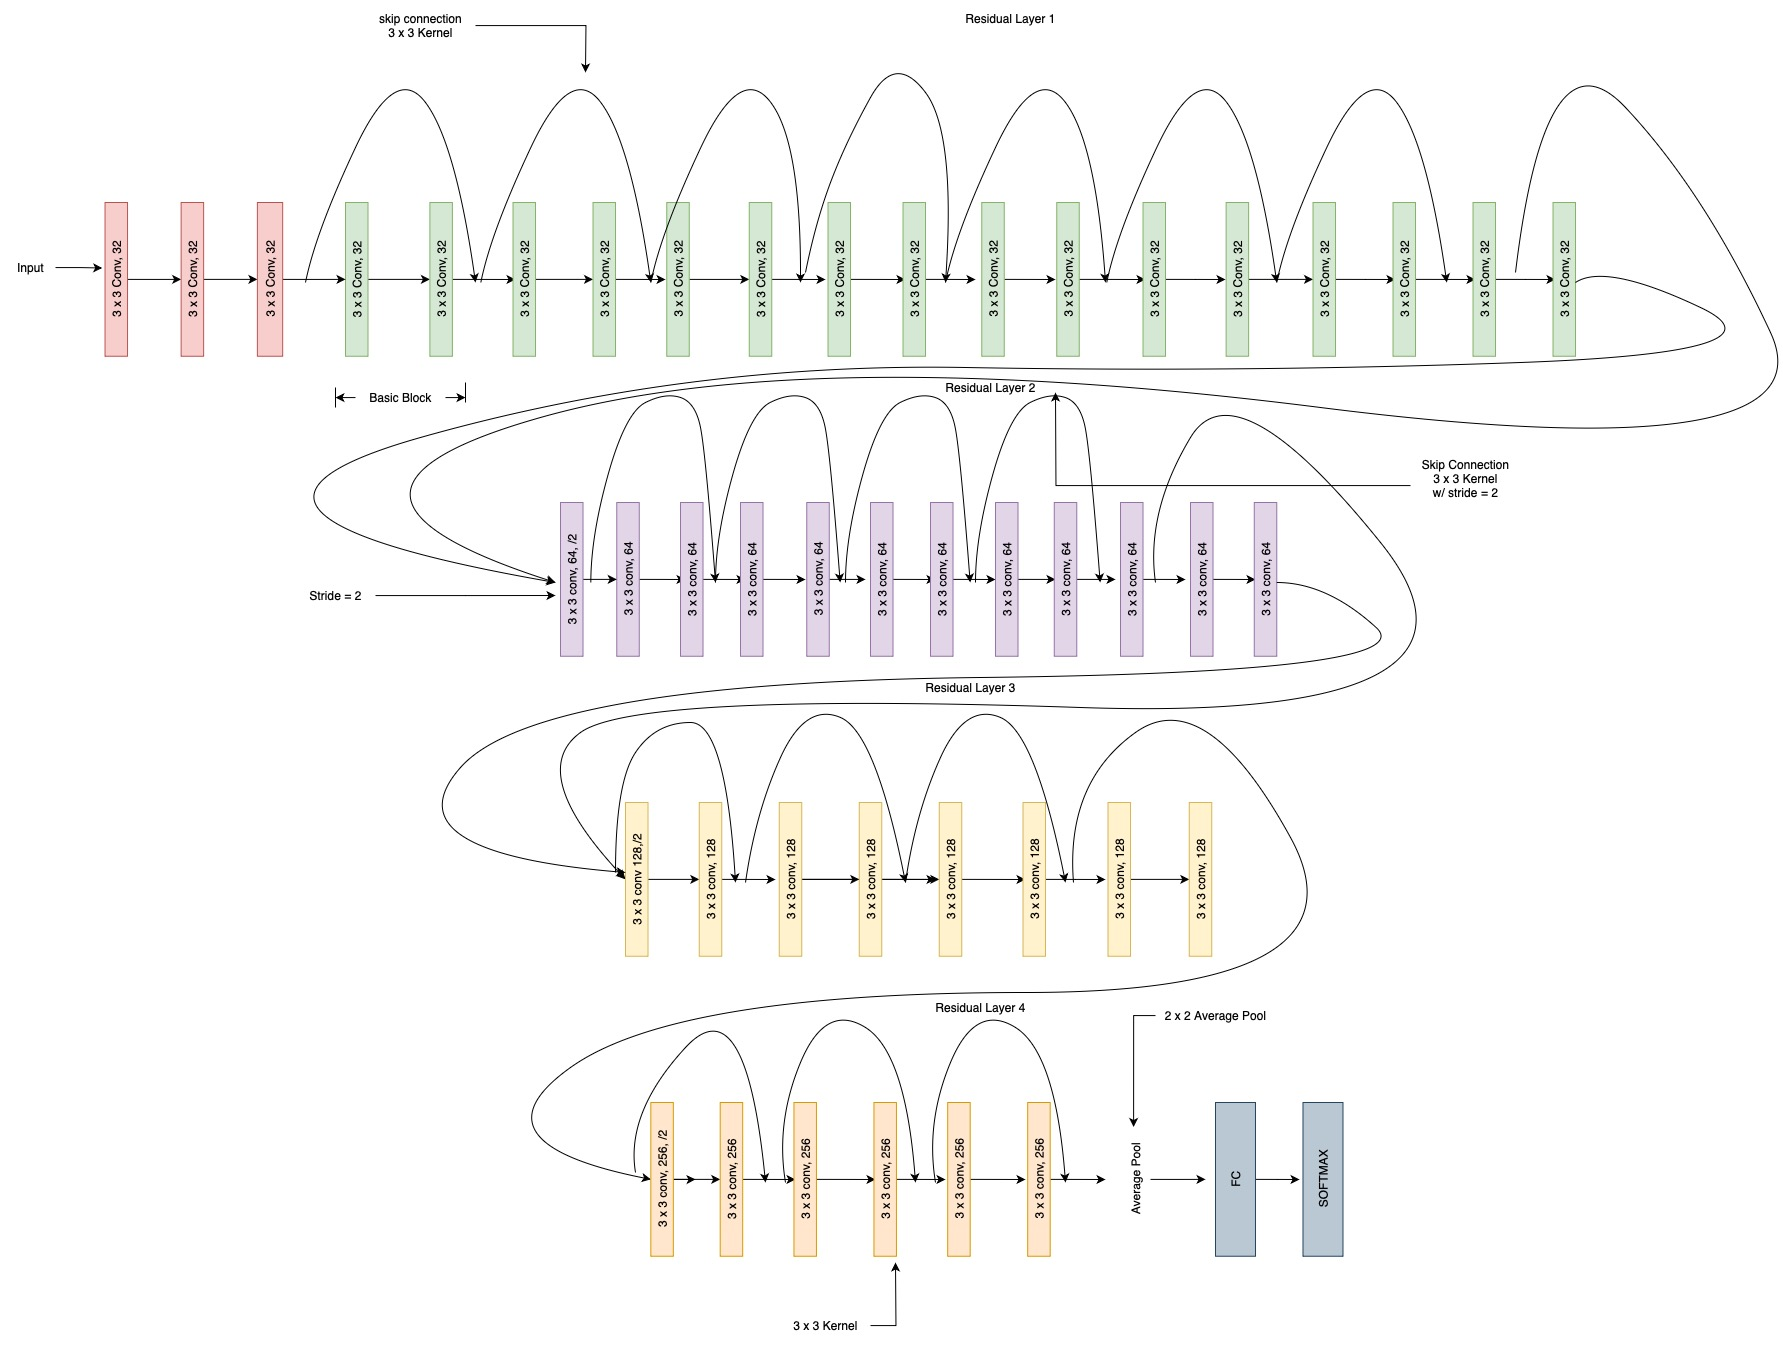
\includegraphics[width=0.5\textwidth]{ArchitectureDiagram.jpg}
We utilized the ResNet-18 architecture, introduced by He et al. \cite{he2016deep} as a starting point due to its proven effectiveness in image classification tasks, particularly on larger datasets like ImageNet. However, the CIFAR-10 dataset presents a unique challenge due to its small image size of 32x32 pixels, in contrast to the 224x224 pixel images the original ResNet models were designed for. To address this, several modifications were made to the network’s architecture.
\begin{enumerate}
    \item \textbf{Adjustment of the First Convolutional Layer: } The first convolutional layer, which originally used 64 channels in ResNet-18, was modified to use only 32 channels. This change was made because the original 64 channels were designed for larger images, and reducing them helped decrease the parameter count, without significantly affecting performance for the smaller CIFAR-10 images.
    \item \textbf{Modification of the Residual Blocks: } The key to ResNet’s success lies in its residual blocks, which allow for deeper networks without suffering from the vanishing gradient problem. To control the number of parameters, the depth and width of these blocks were adjusted. The model’s residual blocks were modified to have fewer filters: instead of the default 64 to 512 filters in four layers, the number of filters was reduced to a range from 32 to 256. Specifically, the architecture employed 4 residual layers with a width ranging from 32 filters to 256 filters, using a consistent kernel size of 3x3 across all layers. This change brought the total parameter count to approximately 4.994 million, staying within the 5 million constraint.
    \item \textbf{Choice of Kernel Size:} The kernel size for all convolutional layers was kept consistent at 3x3, which is a common choice in modern convolutional neural networks. This kernel size provides a good trade-off between computational efficiency and receptive field coverage, ensuring that the model can capture important spatial features in the CIFAR-10 images.
    \item \textbf{Impact of Reducing Depth and Width:} While reducing the number of parameters, particularly the depth and width of the residual blocks \cite{zagoruyko2016wide}, might seem to diminish model capacity, careful experimentation showed that the modified ResNet-18 still performed well on the CIFAR-10 task. However, reducing these parameters also limited the model's ability to learn more complex features, requiring careful tuning to avoid underfitting.
\end{enumerate}

\subsection{Data Augmentation}
To overcome the challenge of having a relatively small dataset, data augmentation was employed to significantly increase the size and diversity of the training data. The CIFAR-10 dataset originally contains 50,000 training images, but by applying several transformation techniques, the dataset size was expanded to over 10 times the original size.
\begin{enumerate}
    \item \textbf{Applied Transformations:} Various augmentations were used to create a more robust and varied training dataset. These included:
        \begin{itemize}
            \item Random Horizontal Flip: The image is flipped horizontally with a 100\% probability, introducing spatial invariance.
            \item Gaussian Blur: A Gaussian blur was applied to simulate blurriness due to various factors like camera motion.
            \item FiveCrop: This transformation crops the image into five sections (four corners and the center), creating more varied data.
            \item ColorJitter: Contrast and brightness were randomly adjusted to simulate different lighting conditions.
            \item Grayscale to RGB Conversion: The image was converted to grayscale and then back to RGB, allowing the model to learn from features that aren't solely dependent on color.
        \end{itemize}
        These transformations increased the dataset's diversity by creating multiple versions of each image. The training set size was increased by generating augmented images, which provided the model with more data to learn from and helped reduce overfitting \cite{perez2017effectiveness}.
    \item \textbf{Dataset Class Customization: }A custom CIFAR10Dataset class was created to handle the original images and apply the transformations. The class ensured that for each image in the CIFAR-10 training set, multiple augmented versions were generated and added to the dataset. This resulted in a significant increase in the number of training examples, making the model more robust and generalizable.
    \item \textbf{Effect of Augmentation on Dataset Size: } By applying up to 10 different augmentations to each image, the total training dataset grew by a factor of 10, which dramatically increased the size of the dataset. This strategy not only increased the amount of data the model trained on but also helped improve generalization performance by introducing additional variability in the training data.
\end{enumerate}

\subsection{Training Strategy}
The training process employed several key techniques to optimize the model’s performance:
\begin{enumerate}
    \item \textbf{Optimizer:} The model was trained using the SGD (Stochastic Gradient Descent) optimizer with a learning rate of 0.1, momentum set to 0.95, and Nesterov acceleration. Weight decay was applied with a value of $4 * 10^{-5}$ to regularize the model and prevent overfitting. The Lookahead optimizer was used in conjunction with SGD, with the hyperparameters $k = 5$ and $\alpha = 0.8$, to improve convergence and enhance the stability of the optimizer during training.
    \item \textbf{Learning Rate Scheduler: }The OneCycleLR scheduler was used with a maximum learning rate of 0.1, which gradually adjusts the learning rate throughout the training process to improve convergence. The scheduler was set for 50 epochs with a 25\% warm-up period, followed by an annealing strategy that uses a cosine decay for the learning rate.
    \item \textbf{Loss Function: } To enhance the model’s robustness, a custom Smooth Cross-Entropy loss function with label smoothing was implemented. Label smoothing reduces overfitting by encouraging the model to output less confident predictions for each class, thereby making the model more generalized.
    \item \textbf{Mixed Precision Training: } Mixed precision training, facilitated by GradScaler from PyTorch, was used to reduce the memory consumption and speed up training by using 16-bit floating-point numbers for the forward and backward passes while maintaining 32-bit precision for the model's weights.
    \item \textbf{Training and Evaluation:} The model was trained for 50 epochs with early stopping based on test accuracy. The model was saved whenever it achieved a new best accuracy on the validation set, ensuring that the best-performing model was preserved.
\end{enumerate}
During the training process, the model's performance on the test set was evaluated at regular intervals to monitor its progress. Early stopping was applied if the test accuracy did not improve significantly over several epochs, thus preventing overfitting and reducing training time.

\subsection{Sequential Training with Learning Rate Adjustment}
To ensure stable convergence and optimal performance, the model was trained over 200 epochs in total, spread across multiple training runs. In each run, the best model weights from the previous run (MWT\_best.pth) were loaded, and the model continued training from that point. This allowed for incremental improvements over successive runs.
\begin{enumerate}
    \item \textbf{Learning Rate Adjustment:} The learning rate was reduced sequentially in four stages during training. This gradual reduction allowed the model to converge more effectively by providing finer adjustments to the weights as training progressed. The learning rate decay was applied to ensure that the model did not overshoot the optimal solution, improving both convergence and final performance.
    \item \textbf{Early Stopping:} Early stopping was implemented to prevent overfitting by monitoring the model's performance on the test set. If the test accuracy did not improve significantly over several epochs, training was halted to avoid unnecessary computations and potential overfitting.
\end{enumerate}

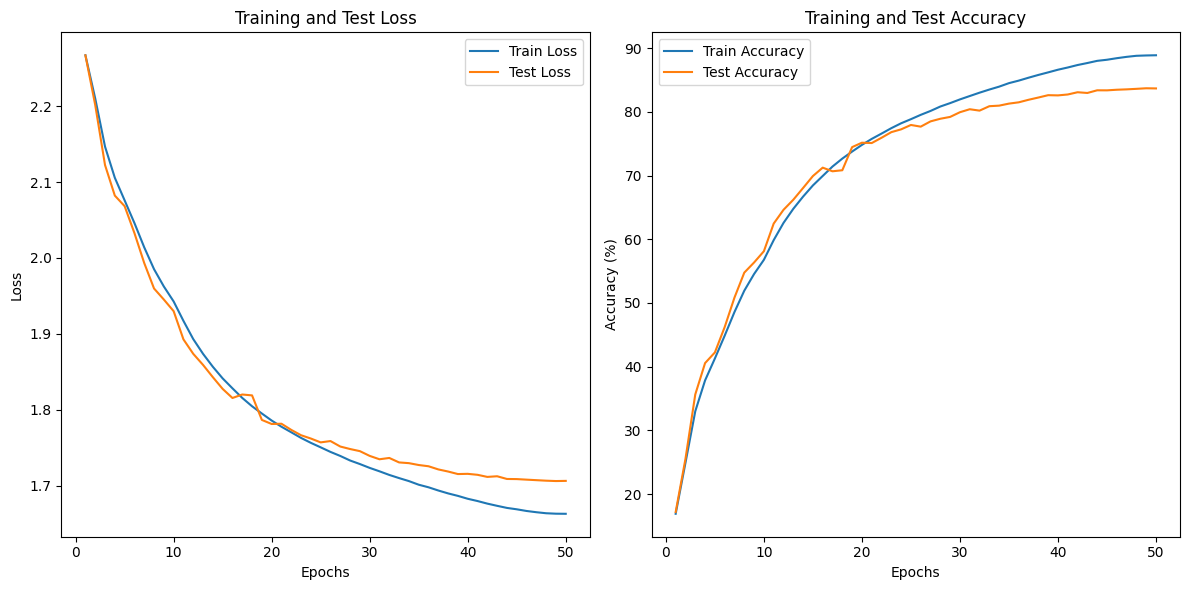
\includegraphics[width=0.5\textwidth]{Training.png}

\subsection{Hyperparameter Tuning with Optuna}
To optimize the model’s performance further, hyperparameter tuning was performed using Optuna, an automated hyperparameter optimization framework \cite{akiba2019optuna}. The goal was to find the best learning rate and weight decay parameters to improve the model's generalization capabilities.
\begin{enumerate}
    \item \textbf{Hyperparameters Tuned:} The learning rate (lr) and weight decay (weight\_decay) were selected as the hyperparameters to be tuned. A logarithmic search space was defined for both parameters:
        \begin{itemize}
            \item Learning Rate (lr): A range from $1*10^{-6}$ to $1*10^{-2}$ was defined, allowing for a wide exploration of learning rates to find the most effective one for the model.
            \item Weight Decay: A range from $1*10^{-6}$ to $1*10^{-4}$ was set to optimize regularization and prevent overfitting.
        \end{itemize}
    \item \textbf{Optuna Setup:} Optuna was used to run 5 trials to search for the optimal combination of these hyperparameters. For each trial, the model was trained using a combination of learning rate and weight decay values suggested by Optuna. The trial returned the negative of the training accuracy to minimize it during optimization.
    \item \textbf{Best Hyperparameters:} After running the optimization, the best trial resulted in the following hyperparameters:
        \begin{itemize}
            \item Learning Rate (lr): 0.00033
            \item Weight Decay: $9.94*10^{-5}$
        \end{itemize}
    \item \textbf{Objective Function:} The objective function used in Optuna evaluated the performance of the model based on these hyperparameters and returned the negative accuracy as the value to minimize.
\end{enumerate}

\subsection{Fine-Tuning with Optimized Hyperparameters}
Once the best hyperparameters were identified using Optuna, the model underwent fine-tuning to further enhance its performance. The goal of this step was to use the optimal learning rate and weight decay to refine the model's weights, leveraging the previously saved best model.
\begin{enumerate}
    \item \textbf{Fine-Tuning Process:} After loading the best weights from the previous run (MW\_best.pth), the model was trained for 5 additional epochs. During these epochs, the learning rate and weight decay parameters found during the Optuna search were applied to ensure optimal convergence.
    \item \textbf{Learning Rate Scheduler:} The OneCycleLR scheduler was used again, with the optimized learning rate and weight decay values, to ensure a smooth learning rate annealing process during the fine-tuning.
    \item \textbf{Saving Best Weights:} At the end of each epoch, the model’s weights were saved if there was an improvement in test accuracy. The fine-tuning helped further optimize the model by making small adjustments to the weights, improving its final performance.
\end{enumerate}

\subsection{Test Time Augmentation (TTA)}
To optimize model performance during testing, Test Time Augmentation (TTA) was applied. TTA involves passing multiple augmented versions of each test image through the model and averaging the predictions. This technique reduces prediction variance and improves accuracy.

The model was loaded with the best pre-trained weights (MWT\_best.pth), and the following transformations were applied during testing: horizontal flip, Gaussian blur, and color jittering (contrast and brightness). Predictions from each augmented version of the image were averaged to obtain the final output.

This process improved the model's robustness and overall test accuracy by averaging over multiple transformations, providing a more stable prediction.

\subsection{Architectural Variations and Challenges}
\begin{enumerate}
    \item \textbf{SE-ResNet:} Initially, experiments were conducted with Squeeze-and-Excitation (SE) blocks, which are designed to improve the representational capacity of the network by re-calibrating the channel-wise feature responses. While SE-ResNet significantly improved model accuracy, it was ultimately discarded due to the project’s constraint on the use of attention \cite{openai2023chatgpt} mechanisms. The use of attention was not allowed in the scope of this project, so the SE blocks were removed, reverting to a standard ResNet structure.
    \item \textbf{Model with Fewer Parameters:} Other experiments included modifying the model further by reducing the width and depth of the network, resulting in fewer parameters. These models performed decently but did not achieve the same level of accuracy as the final ResNet model with the 32-256 filter configuration.
    \item \textbf{Convolutional Layer Modifications:} Another architectural variation involved changing the number of convolutional layers at the beginning of the network. Initially, a single convolutional layer was used. However, as the model struggled to extract sufficient features from the small CIFAR-10 images, the architecture was modified to include multiple convolutional layers. This change helped the model learn more complex features but also increased the number of parameters slightly.
\end{enumerate}


\begin{table}[ht]
    \centering
    \resizebox{\columnwidth}{!}{
    \begin{tabular}{|l|l|l|l|}
    \hline
    \textbf{Model}&\textbf{Params}&\textbf{Train Acc}&\textbf{Test Acc}\\ \hline
    Deep ResNet with Lookahead SGD E:200& 4.994M & 97.94\% & 92.48\% \\ \hline
    SEResNet with SGD and Epoch:50 & 4.996M & 99.78\% & 91.35\% \\ \hline
    Wide ResNet with SGD and Epoch:100 & 4.042M & 92.78\% & 83.28\% \\ \hline
    ResNet with Adam and Epoch:100& 3.572M & 100.0\% & 87.52\% \\ \hline
    ResNet with SGD and Epoch:40& 3.572M & 87.43\% & 78.82\% \\ \hline
    \end{tabular}
    }
    \label{table:models_comparison}
\end{table}
\vspace{-0.5cm}
\subsection{Lessons Learned}
\begin{enumerate}
    \item \textbf{Balancing Performance and Efficiency:} The process taught me the importance of balancing network depth and width, especially in the context of a parameter budget. While deep networks tend to perform better \cite{simonyan2014very}, reducing the width and depth too much can lead to underfitting and poor accuracy. Finding the optimal configuration required several trials, each focusing on different layers of the ResNet.
    \item \textbf{Training Techniques Matter:} The combination of advanced techniques such as the Lookahead optimizer, OneCycleLR scheduler, and mixed precision training helped achieve good results without overfitting. These strategies allowed the model to converge faster and generalize well to the test data.
    \item \textbf{Model Size Constraints:} Designing a model with a strict parameter constraint is challenging but rewarding. It forces the practitioner to think creatively about optimizing the architecture and training strategies. The modified ResNet-18 with under 5 million parameters demonstrated that a well-tuned, smaller network can achieve competitive performance, making it suitable for resource-constrained environments.
\end{enumerate}
\section{Results and Discussion}
\label{sec:results}
The final model, after undergoing hyperparameter tuning and fine-tuning, achieved a train accuracy of 97.94\% on augmented data and test accuracy of 92.48\% on the CIFAR-10 test dataset. The model architecture used was a modified version of ResNet-18, where the first convolutional layer was adjusted to 32 channels (instead of 64) to better fit the smaller 32x32 image size of the CIFAR-10 dataset. The architecture was further modified by reducing the depth and width of the residual blocks, resulting in a total of approximately 4.994 million parameters. Through careful hyperparameter tuning using Optuna and subsequent fine-tuning, the model's performance was further optimized, achieving a strong balance between accuracy and computational efficiency.

\bibliographystyle{aaai24}
\bibliography{references} 
\end{document}
